\documentclass{standalone}
\usepackage{tikz}
\usetikzlibrary{patterns, positioning}

\begin{document}
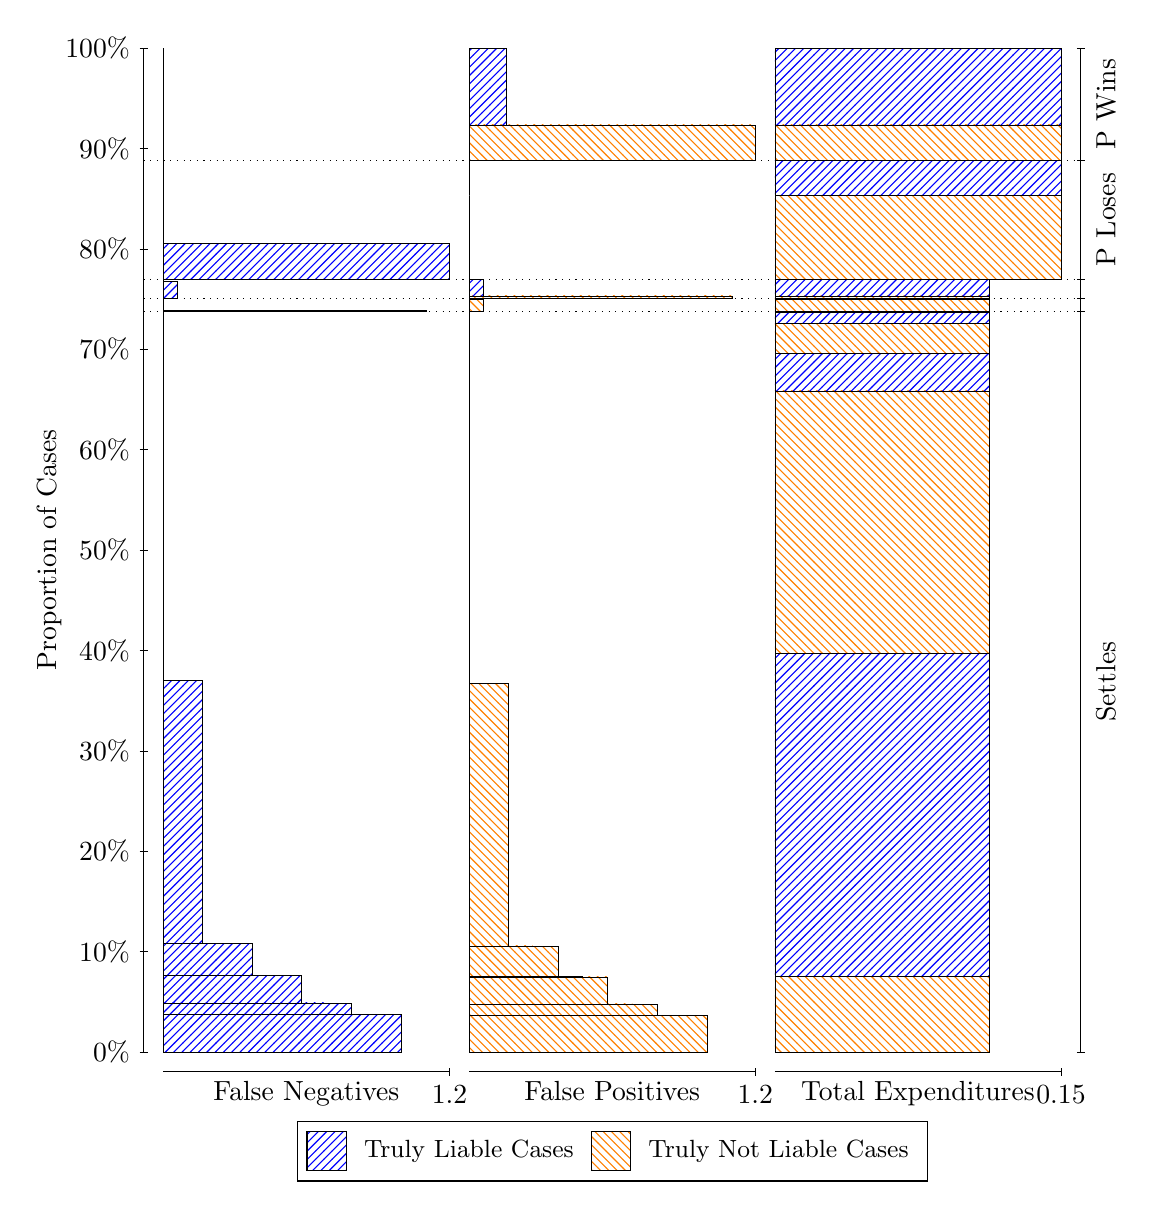
\begin{tikzpicture}
\draw[black, very thin] (1.5,1.75) -- (1.5,14.5);
\node[rotate=90, anchor=center] at (0.3, 8.125) {Proportion of Cases};
\draw[black, very thin] (1.45,1.75) -- (1.55,1.75);
\node[anchor=east] at (1.45, 1.75) {0\%};
\draw[black, very thin] (1.45,3.025) -- (1.55,3.025);
\node[anchor=east] at (1.45, 3.025) {10\%};
\draw[black, very thin] (1.45,4.3) -- (1.55,4.3);
\node[anchor=east] at (1.45, 4.3) {20\%};
\draw[black, very thin] (1.45,5.575) -- (1.55,5.575);
\node[anchor=east] at (1.45, 5.575) {30\%};
\draw[black, very thin] (1.45,6.85) -- (1.55,6.85);
\node[anchor=east] at (1.45, 6.85) {40\%};
\draw[black, very thin] (1.45,8.125) -- (1.55,8.125);
\node[anchor=east] at (1.45, 8.125) {50\%};
\draw[black, very thin] (1.45,9.4) -- (1.55,9.4);
\node[anchor=east] at (1.45, 9.4) {60\%};
\draw[black, very thin] (1.45,10.675) -- (1.55,10.675);
\node[anchor=east] at (1.45, 10.675) {70\%};
\draw[black, very thin] (1.45,11.95) -- (1.55,11.95);
\node[anchor=east] at (1.45, 11.95) {80\%};
\draw[black, very thin] (1.45,13.225) -- (1.55,13.225);
\node[anchor=east] at (1.45, 13.225) {90\%};
\draw[black, very thin] (1.45,14.5) -- (1.55,14.5);
\node[anchor=east] at (1.45, 14.5) {100\%};

\draw[black, very thin] (13.4,1.75) -- (13.4,14.5);
\draw[black, very thin] (13.35,1.75) -- (13.45,1.75);
\node[anchor=west] at (13.35, 1.75) {};
\draw[black, very thin] (13.35,11.154) -- (13.45,11.154);
\node[anchor=west] at (13.35, 11.154) {};
\draw[black, very thin] (13.35,11.321) -- (13.45,11.321);
\node[anchor=west] at (13.35, 11.321) {};
\draw[black, very thin] (13.35,11.566) -- (13.45,11.566);
\node[anchor=west] at (13.35, 11.566) {};
\draw[black, very thin] (13.35,13.075) -- (13.45,13.075);
\node[anchor=west] at (13.35, 13.075) {};
\draw[black, very thin] (13.35,14.5) -- (13.45,14.5);
\node[anchor=west] at (13.35, 14.5) {};

\draw[black, very thin, pattern color=blue, pattern=north east lines] (1.75,1.75) rectangle (4.7712,2.2264);
\draw[black, very thin, pattern color=blue, pattern=north east lines] (1.75,2.2264) rectangle (4.4553,2.2296);
\draw[black, very thin, pattern color=blue, pattern=north east lines] (1.75,2.2296) rectangle (4.1393,2.3684);
\draw[black, very thin, pattern color=blue, pattern=north east lines] (1.75,2.3684) rectangle (3.8234,2.3729);
\draw[black, very thin, pattern color=blue, pattern=north east lines] (1.75,2.3729) rectangle (3.5074,2.7197);
\draw[black, very thin, pattern color=blue, pattern=north east lines] (1.75,2.7197) rectangle (3.1915,2.727);
\draw[black, very thin, pattern color=blue, pattern=north east lines] (1.75,2.727) rectangle (2.8755,3.1278);
\draw[black, very thin, pattern color=blue, pattern=north east lines] (1.75,3.1278) rectangle (2.5596,3.1289);
\draw[black, very thin, pattern color=blue, pattern=north east lines] (1.75,3.1289) rectangle (2.2437,6.471);
\draw[black, very thin, pattern color=orange, pattern=north west lines] (1.75,6.471) rectangle (1.75,11.154);
\draw[black, very thin, pattern color=blue, pattern=north east lines] (1.75,11.154) rectangle (5.0871,11.169);
\draw[black, very thin, pattern color=orange, pattern=north west lines] (1.75,11.169) rectangle (1.75,11.321);
\draw[black, very thin, pattern color=blue, pattern=north east lines] (1.75,11.321) rectangle (1.9277,11.535);
\draw[black, very thin, pattern color=orange, pattern=north west lines] (1.75,11.535) rectangle (1.75,11.566);
\draw[black, very thin, pattern color=blue, pattern=north east lines] (1.75,11.566) rectangle (5.3833,12.016);
\draw[black, very thin, pattern color=orange, pattern=north west lines] (1.75,12.016) rectangle (1.75,13.075);
\draw[black, very thin, pattern color=orange, pattern=north west lines] (1.75,13.075) rectangle (1.75,13.525);
\draw[black, very thin, pattern color=blue, pattern=north east lines] (1.75,13.525) rectangle (1.75,14.5);
\draw[black, very thin, pattern color=orange, pattern=north west lines] (5.6333,1.75) rectangle (8.6545,2.212);
\draw[black, very thin, pattern color=orange, pattern=north west lines] (5.6333,2.212) rectangle (8.3386,2.2141);
\draw[black, very thin, pattern color=orange, pattern=north west lines] (5.6333,2.2141) rectangle (8.0226,2.3567);
\draw[black, very thin, pattern color=orange, pattern=north west lines] (5.6333,2.3567) rectangle (7.7067,2.3609);
\draw[black, very thin, pattern color=orange, pattern=north west lines] (5.6333,2.3609) rectangle (7.3908,2.7041);
\draw[black, very thin, pattern color=orange, pattern=north west lines] (5.6333,2.7041) rectangle (7.0748,2.7093);
\draw[black, very thin, pattern color=orange, pattern=north west lines] (5.6333,2.7093) rectangle (7.0748,2.7125);
\draw[black, very thin, pattern color=orange, pattern=north west lines] (5.6333,2.7125) rectangle (6.7589,3.0936);
\draw[black, very thin, pattern color=orange, pattern=north west lines] (5.6333,3.0936) rectangle (6.4429,3.0967);
\draw[black, very thin, pattern color=orange, pattern=north west lines] (5.6333,3.0967) rectangle (6.127,6.4331);
\draw[black, very thin, pattern color=blue, pattern=north east lines] (5.6333,6.4331) rectangle (5.6333,11.154);
\draw[black, very thin, pattern color=orange, pattern=north west lines] (5.6333,11.154) rectangle (5.8111,11.306);
\draw[black, very thin, pattern color=blue, pattern=north east lines] (5.6333,11.306) rectangle (5.6333,11.321);
\draw[black, very thin, pattern color=orange, pattern=north west lines] (5.6333,11.321) rectangle (8.9705,11.353);
\draw[black, very thin, pattern color=blue, pattern=north east lines] (5.6333,11.353) rectangle (5.8111,11.566);
\draw[black, very thin, pattern color=orange, pattern=north west lines] (5.6333,11.566) rectangle (5.6333,12.626);
\draw[black, very thin, pattern color=blue, pattern=north east lines] (5.6333,12.626) rectangle (5.6333,13.075);
\draw[black, very thin, pattern color=orange, pattern=north west lines] (5.6333,13.075) rectangle (9.2667,13.525);
\draw[black, very thin, pattern color=blue, pattern=north east lines] (5.6333,13.525) rectangle (6.1072,14.5);
\draw[black, very thin, pattern color=orange, pattern=north west lines] (9.5167,1.75) rectangle (12.242,2.7093);
\draw[black, very thin, pattern color=blue, pattern=north east lines] (9.5167,2.7093) rectangle (12.242,6.8085);
\draw[black, very thin, pattern color=orange, pattern=north west lines] (9.5167,6.8085) rectangle (12.242,10.145);
\draw[black, very thin, pattern color=blue, pattern=north east lines] (9.5167,10.145) rectangle (12.242,10.621);
\draw[black, very thin, pattern color=orange, pattern=north west lines] (9.5167,10.621) rectangle (12.242,11.006);
\draw[black, very thin, pattern color=blue, pattern=north east lines] (9.5167,11.006) rectangle (12.242,11.148);
\draw[black, very thin, pattern color=orange, pattern=north west lines] (9.5167,11.148) rectangle (12.242,11.151);
\draw[black, very thin, pattern color=blue, pattern=north east lines] (9.5167,11.151) rectangle (12.242,11.154);
\draw[black, very thin, pattern color=orange, pattern=north west lines] (9.5167,11.154) rectangle (12.242,11.306);
\draw[black, very thin, pattern color=blue, pattern=north east lines] (9.5167,11.306) rectangle (12.242,11.321);
\draw[black, very thin, pattern color=orange, pattern=north west lines] (9.5167,11.321) rectangle (12.242,11.353);
\draw[black, very thin, pattern color=blue, pattern=north east lines] (9.5167,11.353) rectangle (12.242,11.566);
\draw[black, very thin, pattern color=orange, pattern=north west lines] (9.5167,11.566) rectangle (13.15,12.626);
\draw[black, very thin, pattern color=blue, pattern=north east lines] (9.5167,12.626) rectangle (13.15,13.075);
\draw[black, very thin, pattern color=orange, pattern=north west lines] (9.5167,13.075) rectangle (13.15,13.525);
\draw[black, very thin, pattern color=blue, pattern=north east lines] (9.5167,13.525) rectangle (13.15,14.5);
\draw[black, dotted] (1.5,11.154) -- (13.4,11.154);
\draw[black, dotted] (1.5,11.321) -- (13.4,11.321);
\draw[black, dotted] (1.5,11.566) -- (13.4,11.566);
\draw[black, dotted] (1.5,13.075) -- (13.4,13.075);
\draw[black, very thin] (1.75,1.5) -- (5.3833,1.5);
\node[anchor=north] at (3.5667, 1.5) {False Negatives};
\draw[black, very thin] (5.3833,1.45) -- (5.3833,1.55);
\node[anchor=north] at (5.3833, 1.45) {1.2};

\draw[black, very thin] (5.6333,1.5) -- (9.2667,1.5);
\node[anchor=north] at (7.45, 1.5) {False Positives};
\draw[black, very thin] (9.2667,1.45) -- (9.2667,1.55);
\node[anchor=north] at (9.2667, 1.45) {1.2};

\draw[black, very thin] (9.5167,1.5) -- (13.15,1.5);
\node[anchor=north] at (11.333, 1.5) {Total Expenditures};
\draw[black, very thin] (13.15,1.45) -- (13.15,1.55);
\node[anchor=north] at (13.15, 1.45) {0.15};

\node[black, centered, rotate=90] at (13.72, 6.4521) {Settles};


\node[black, centered, rotate=90] at (13.72, 12.321) {P Loses};
\node[black, centered, rotate=90] at (13.72, 13.788) {P Wins};

\draw (7.449999999999999,1.5) node[draw=none] (baseCoordinate) {};
\begin{scope}[align=center]
        \matrix[scale=0.5, draw=black, below=0.5cm of baseCoordinate, nodes={draw}, column sep=0.1cm]{
            \node[rectangle, draw, minimum width=0.5cm, minimum height=0.5cm, pattern=north east lines, pattern color=blue] {}; &
            \node[draw=none, font=\small] (B) {Truly Liable Cases}; &
            \node[rectangle, draw, minimum width=0.5cm, minimum height=0.5cm, pattern=north west lines, pattern color=orange] {}; &
            \node[draw=none, font=\small] (B) {Truly Not Liable Cases}; \\
            };
\end{scope}

\end{tikzpicture}
\end{document}